\documentclass[conference]{IEEEtran}
\IEEEoverridecommandlockouts
% The preceding line is only needed to identify funding in the first footnote. If that is unneeded, please comment it out.
\usepackage{cite}
\usepackage{amsmath,amssymb,amsfonts}
\usepackage{algorithmic}
\usepackage{graphicx}
\usepackage{textcomp}
\usepackage{xcolor}
\usepackage{listings}
\def\BibTeX{{\rm B\kern-.05em{\sc i\kern-.025em b}\kern-.08em
    T\kern-.1667em\lower.7ex\hbox{E}\kern-.125emX}}
\begin{document}

\title{Szakdolgozati beszámoló\\

\thanks{}
}

\author{\IEEEauthorblockN{Pekár Mihály}
\IEEEauthorblockA{\textit{PTI bsc.} \\
\textit{Eszterházy Károly Egyetem}\\
Eger, Magyarország \\
mpekar55@gmail.com}
}

\maketitle

\begin{abstract}
Ebben a dokumentumban arról fogok írni, hogy a jelenlegi félévben milyen feladatokat tudtam teljesíteni a szakdolgozatom megírásában illetve, hogy milyen nehézségekbe ütköztem ezalatt. Továbbá azt is befogom még mutatni, hogy mik várnak még rám a szakdolgozatom befejeztéig. 
\end{abstract}

\begin{IEEEkeywords}
iktatás, szakdolgozat, grpc, mysql, protobuffer
\end{IEEEkeywords}

\section{Bevezetés}
Ebben a félévben szakdolgozatom írásánál a legtöbb időt az adatbázis elkészítésére fordítottam. Sok nehézségekbe ütköztem közben. A legnagyobb hátráltatás az volt, hogy megbeszélések soha nem jöttek össze a munkáltatómmal ha mégis nem sok időnk volt alaposan átbeszélni. Miután ez összejött az adatbázis struktúra kialakításához kezdtem ahol az iktatókönyvnek a törlésével elég sokat küzdöttem. Majd jött Protobuffer fájl elkészítése ahol egyenlőre bejelentkezés, kijelentkezés és a regisztrálásnak az rpc hívásait készítettem el. A továbbiakban még elkészítettem c\#-ban a server-t és a klienst ahol implementáltam a protobuffer-ben elkészített rpc call-okat. A login teljesen készlet. 
\section{Féléves munka bemutatása}

\subsection{\textbf{Adatbázis tervezése és megvalósítása}}
Az adatbázisnak a megtervezésekor mindent információt figyelembe vettem amit az igényfelmérés során összegyűjtöttem. Reményeim szerint nem fog kelleni sok mindent újra tervezni mikor csinálom a gRPC szervert illetve a felhasználó felületet. Amit már biztosan tudok, hogy az adatbázisban még van egy probléma méghozzá a partnereknek a tárolása amit még újra kell gondolnom.
\\
\subsubsection{\textbf{Táblák}}
\begin{figure}[htbp]
	\centerline {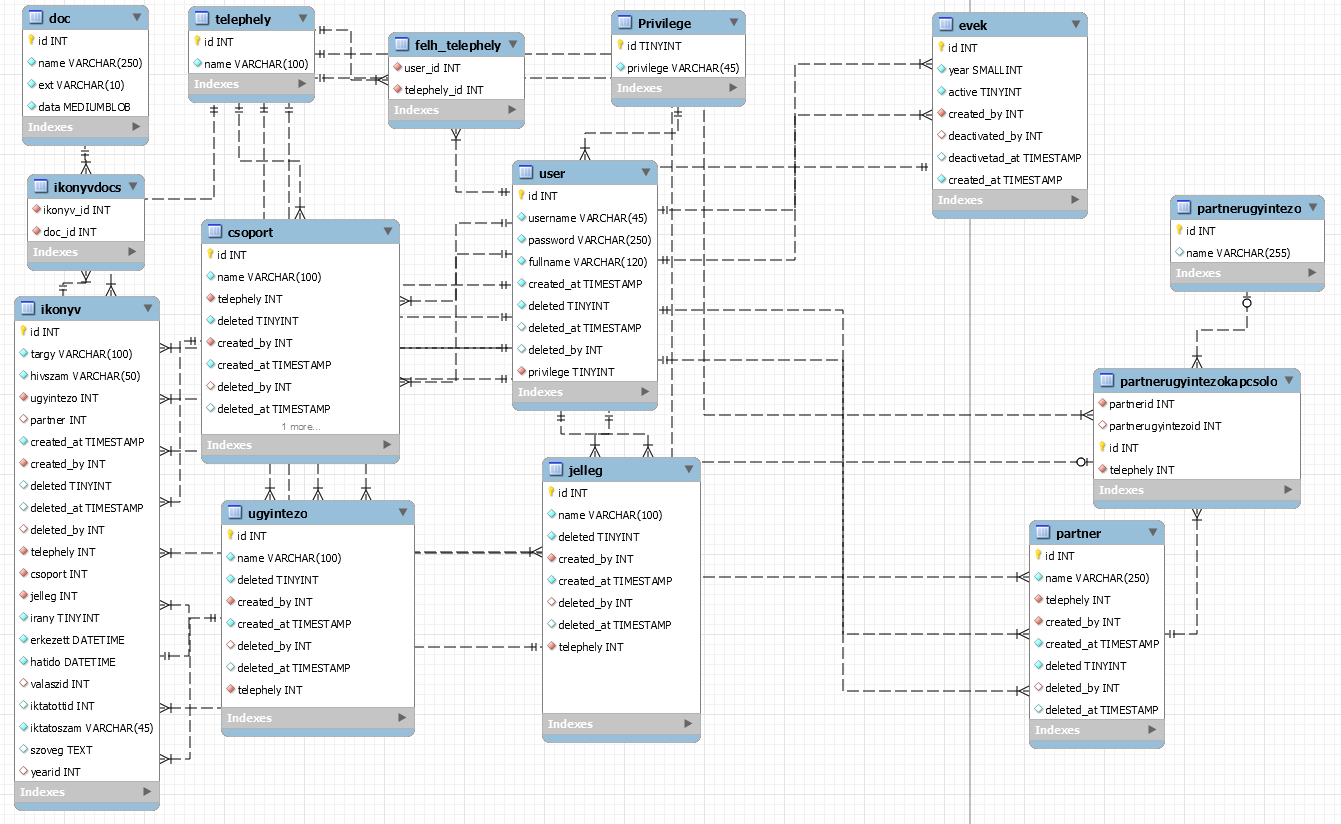
\includegraphics[width=8cm,height=8cm,keepaspectratio]{adatbazis.png}}
	\caption{Adatbázis képe mysql workbenchben programban}
	\label{fig1}
\end{figure}
\begin{itemize}
	\item Évek:
	Az aktív évet jeleníti meg a programban, hogy melyik évre iktatunk. Év zárása után már nem lehet arra az évre iktatni.
	\item User tábla:
	A programot használó dolgozók adatait tartalmazza. Három oszlopból áll. Felhasználónév aminek a maximális mérete 45 karakterhosszú. Jelszó ami SHA1 kódolással lesz eltárolva, illetve a felhasználó teljese neve.
	\item Privilege:
	A felhasználó jogosultásgi szintje a programban. Lehet Admin és User. Az admin jogosultsággal rendelkezők a törzseket szabadon szerkeszthetik, felhasználókat adhatnak , módosíthatnak vagy törölhetnek a rendszerben illetve "törölhetnek" iktatásokat.
	Míg a sima felhasználó iktatáson kívül még partnert, partner ügyintézőt és ügyintézőket tud csak hozzáadni a rendszerhez.
	\item Telephely:
	Ez jelöli, hogy az adat az melyik telephelyhez tartozik az adatbázisban. Ez vonatkozik az iktatásra és a törzsadatokra egyaránt.	
	\item Felhtelephely:	
	Minden felhasználóhoz tartozik egy vagy több telephely ahová tud iktatni vagy törzs adatokat rögzíteni. 
	\item Partner:	
	Azokat a partnereket tartalmazza akiket a
	\item Partnerügyintéző:
	A megadott partnerhez tartozó ügyintézőket tartalmazza
	\item Partnerügyintéző kapcsoló:
	Az a személy, intézmény vagy cég aki küldte az iratot. Munkaszerződéseknél a partner a dolgozó nevét jelöli. Lehet például E-on, Járási hivatal..stb. Ennek a táblának az id-je fog idegen kulcsként megjelenni az iktatásban.
	\item Csoport
	Az iratok azon típusait jelöli, amely egységhez kapcsolódik az iktatandó anyag. Például Ellátotti, Főzőkonyha, Munkaügy.
	\item Jelleg
	A dokumentum formai megjelenésének megadása. Ez lehet e-mail, küldemény, fax, levél, munkaügyi irat.
	\item Ügyintéző	
	Ez a szervezeten belüli dolgozó kollégára utal, hogy ezt az ügyet vagy iratot ki intézi.
	\item Doc
	Itt tároljuk az iktatásokhoz feltöltött állományokat mediumblobban. Illetve eltároljuk még annak nevét és a kiterjesztését is. Lehet Pdf,JPG,PNG,XLSX,DOCX...stb.
	\item Ikonyv docs
	Az adott iktatáshoz tartozó dokumentum.
	\item Ikonyv
	Ez maga az iktató könyv. Ha bejön egy irat vagy kimegy azt itt lesz rögzítve. Az iktatószámot tárolt eljárással fogom előállítani ami a megadott adatok alapján fog generálódni. Egy példa: B-SZ/R/3/2019 Ennek felépítése
	\begin{itemize}
		\item Az első karakteret az határozza meg, hogy K - kimenő vagy B - bejövő
		\item A második karakter a jellege határozza meg SZ pl szerződés.
		\item A harmadik karakter a telephely jelöli pl. R - Rákóczi, V- Vajda stb..
		\item A negyedik karakter sorozat a sorszám ami lehet kötőjeles Pl. B-SZ/R/3-1/2019 vagy B-SZ/R/3-1-1/2019 a válaszokhoz mérve.
		\item Az utolsó rész pedig az évet jelöli.
		
	\end{itemize}
	Az iktatószám generálása után el is lesz tárolva.
	
\end{itemize}
\subsubsection{\textbf{Nézetek}}
Egyenlőre három nézetem van. Első a creatIktSzam ahol a iktató könyv tábla összes idegen kulcsa össze van kapcsolva a táblájával és ezekből össze állítja az aktuális iktató könyv iktatószámát. A második a currentYearIkonyv itt lekérem az aktuális év iktatásait olyan formában amiben majd a programban kelleni fog. Illetve az utolsó a prevYearIkonyv ami hasonló a currentYearIkonyvhöz de itt saját kezűleg kell paraméterezni az évet.


\subsubsection{\textbf{Tárolt eljárások}}

Minden kérést amit lehetett tárolt eljárásba tettem. Ezzel is megakadályozva az SQL injectionnek a lehetőségét. Összesen 39 darab lett belőlük, de ezeknek a száma valószínűleg csak növekedni fog az iktató program fejlesztése során mivel előfordulhatnak olyan lekérdezések amikre még nem gondoltam a tervezés során.
Pár fontosabb eljárást fogok csak bemutatni, mivel a nagy része csak az adatok megfelelő módosításáról, törléséről és hozzáadásáról szól. A legfontosabbak a következők.
AddRootIkonyv, AddSubIkonyv, DelIkonyv, setDeletedByValaszID, getNextIktatottID, getIkonyvek. Ezek okozták a legtöbb fejtörést a számomra.
 
\textbf{AddRootIkonyv:}
	Bemenete az iktatóhoz szükséges adatok mint a Tárgy, Hivatkozási szám, Ügyintéző id-je, PartnerÜgyintézőkapcsoló id-je, stb... Első lépésben lekérem az aktuális évet, erre azért van szükség hogy az iktatószámhoz hozzátudjam adni.(Az aktuális év nem feltétlenül egyezik meg az aktuális dátummal). Második lépésben lekérem a következő Id-t. Mivel több telephely is szerepel a táblázatban ezért van erre szükség így mindegyik telephelyen a számozás konzisztens marad illetve még a válasz iktatások is bekavarnának a sima ID-ba. Harmadik lépésben hozzáadom az uj iktató könyvet még iktatószám nélkül. Negyedik lépésben lekérem az ő ID-ját a táblából így az generateIktSzam viewval le tudom generáltati az iktatószámát és hozzáadni az iktatókönyvhöz. Utolsó lépésben vissza adom az új iktatásnak az id-ját így ha kell le tudom egyből kérdezni. Ez lehet változni fog mivel valószínűleg csak az iktatószámra lesz szükségem a hozzáadás során.

\textbf{AddSubIkonyv:}
 	A bemenete hasonló az szülőhöz de itt még paraméterként várom annak az iktatókönyvnek az id-jet amihez ez az iktatás kapcsolódik. A lépések ugyan azok mint a szülő ikönyvnél, de itt mikor lekérem az iktatókönyvnek a következő id-jet még hozzá kell tennem a szülőnek az ID-jét is. Iktatószám generálása kicsit másképp történik. Először lekérem az szülő  iktatószámát és azt átalakítva mentem el az ikönyv táblában.
 	
\textbf{DelIkonyv:}
 Az iktató könyv törlése elég macerás dolog. Mivel a könyvnek lehetnek gyermek iktatásai és a gyermek iktatásnak is lehetnek gyermek iktatásai, ezért erre oda kell figyelnem, hogy ha az egyik szülőt kiszedjük a fa struktúrából akkor az összes gyermeket is "törölje". Természetesen végleges törlést nem csinálunk csak a deleted flaget 1-re állítjuk.
 Bemenő paraméterek: az iktató könyvnek az id-je és a felhasználónak az id-je. Igazából nem csinál mást csak meghivja a setDeletedByValaszID-t a bemenő paraméterekkel.

\textbf{setDeletedByValaszID:}
 A bemenő paraméterek ugyan azok mint a DelIkonyvnek. Első lépésben megnézzük, hogy az iktatásnak vannak-e gyermekei, ha nincs akkor a flaget 1-re állítjuk ha van akkor a következő lépéseket kezdjük. Amíg van gyermeke addig kiválasztjuk az első gyermeket. A gyermek delete flagjét 1-re állítjuk és meghívjuk ezt az eljárást a jelenlegi gyermek iktatásra. A legvégén az eredetileg meghívott iktatókönyvnek is a flag-jét 1-re állítjuk. 
 
 \textbf{getNextIktatottID:}
 A bemenete a telephelynek az id-je és hogy ha van akkor a szülőnek az id-je. Először meg nézem hogy a válasz id null-e ha igen akkor a következő selectet meghívom:  select IFNULL(MAX(iktatottid),0)+1 into nextiktatottid from ikonyv where telephely = telephely\_b and valaszid is null\;
 Viszont ha van válaszid akkor ugyan ezt a selectet hívom meg csak a where feltétel módosul.
 
 \textbf{getIkonyvek:}
 Bemente a userid így kitudom keresni hogy a felhasználóhoz melyek azok a telephelyek amik hozzá tartoznak és csak azokat fogom lekérni. Egy ilyet még írnom kell a prevYearIkonyv-re is de ahhoz még kelleni fog bemenő paraméternek az év. Illetve a lapozáshoz még fog kelleni egy tól-ig paraméter is.


\subsection{\textbf{gRPC és Protocol Buffers}}
\textbf{Grpc:}

A gRPC rekurzív mozaik szó. A jelentése gRPC Remote Procedure Call. A google fejlesztette 2015-ben. Nyílt forráskódú. Két főrészből áll. Első a gRPC protokoll és a ProtocolBuffer azaz a adat szerializáció. A protokoll http2 alapokon működik és ki is használja azok előnyeit. Például fejléc tömörítés, egyetlen folyamatos TCP kapcsolat, megszakító és időtúllépés contract a kliens és a szerver között. A gRPC RPC tipusa: Unáris: Azaz a kliens küld egy requestet és a szerver válaszol arra. Kliens streaming RPC: Ahol a kliens több üzenetet küld ezt megvárja a szerver és ha a kliens végzett a szerver válaszol egy válaszban. Server Streaming RPC: Ami a Kliensnek az ellentettje. És van a bidirectional streaming rpc ahol a kliens és a szerver egymástól függetlenül tudnak több üzenetet küld egymásnak. 

\textbf{Protocol Buffer:}
A protocol buffer egy nyelv, platform semleges protokoll ami az adatok szerializációjáért felel. Sokkal egyszerűbb, hatékonyabb és flexibilisebb mint egy XML struktúra és könnyebben olvasható is. Két részből áll az egyik a Message a másik a Service amiben az rpc-k találhatóak. Megtalálhatóak benne skalár típusok Pl.: int32,int64,double,string stb \dots 

\subsubsection{Message}
A message egy üzenet ami az rpc híváskor adható meg paraméterként illetve ilyen üzeneteket tud visszaküldeni a szerver. Itt lehet a classokat kialakítani illetve egyéb segéd osztályokat. Illetve az rpc hivásoknál nem lehet üres a metódus ezért létre kell hozni egy EmptyMessaget aminek nincs semmi mezője és ezt belerakni. Nekem egyenlőre van a user-hez kapcsolodó rpc-k és messagek vannak kialakítva. Ami LoginMessage, Answer, User, Privilege. Az LoginMessage tartalmaz egy string felhasználó nevet és egy string password mezőt. Ezt fogja a kliens elküldeni a szerver felé a szerver majd válaszol egy User requesttel. Az Answer tartalmaz egy bool error és egy string message mezőt. Ami a kijelentkezéskor és a regisztrációkor használatos. 


\subsubsection{Service}

A service nem más mint azoknak a rpc metódusoknak gyűjtőneve amit használni szeretnénk a grpc-kor. Több service is megadható, de ki kell választanunk szerver indításakor, hogy melyiket használja. Egyenlőre három rpc-m van a Login, Logout,Register,ModifyUser. Ezek lesznek a userrel való műveletek. Mint látszódik is a login egy LoginMessaget vár a többi User Messaget. és a Loginon kívül más nem küld vissza User Message-t.

\begin{lstinputlisting}{iktato.proto}
	
\end{lstinputlisting}
\subsection{\textbf{Szerver és Kliens}}

\subsubsection{Szerver}


\subsubsection{Kliens}
\begin{figure}[htbp]
	\centerline {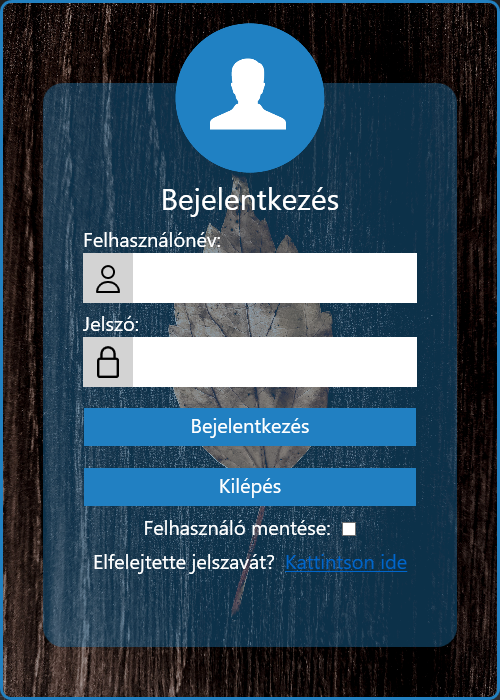
\includegraphics[height=8cm,keepaspectratio]{login.png}}
	\caption{A kliens login felülete.}
	\label{fig1}
\end{figure}

\section*{Feladatok, tervek és azok kivitelezése a szakdolgozat befejezéséig.}
Lényegében az egész egész szoftver fejlesztése még hátra van,de szerencsére a caliburn.micro és a gRPC segítségével nem lesz nehéz időben ezt befejezni. Tervbe van még véve, hogy TDD-ben lesz a fejlesztés és egy loggolás server és kliens oldalon is. Illetve, hogy a RPC hívsoknál várni fogok még valami token -t is ami validálja a usert hogy meghívhatja e az adott metódust.


\section*{Eredmények}
Ebben a félévben elértem, hogy az adatbázisommal ne nagyon kelljen foglalkoznom már a fejlesztés során illetve sikerült összehozni egy körülbelüli képet a munkáltatómmal, hogy hogy is nézzen ki a program. Sikerült SSL titkosítás implementálása, hogy a gRPC szerver és a kliens ne egy insecure channelen kommunikáljanak.

\begin{thebibliography}{00}
\bibitem{b1} G. Eason, B. Noble, and I. N. Sneddon, ``On certain integrals of Lipschitz-Hankel type involving products of Bessel functions,'' Phil. Trans. Roy. Soc. London, vol. A247, pp. 529--551, April 1955.
\bibitem{b2} J. Clerk Maxwell, A Treatise on Electricity and Magnetism, 3rd ed., vol. 2. Oxford: Clarendon, 1892, pp.68--73.
\bibitem{b3} I. S. Jacobs and C. P. Bean, ``Fine particles, thin films and exchange anisotropy,'' in Magnetism, vol. III, G. T. Rado and H. Suhl, Eds. New York: Academic, 1963, pp. 271--350.
\bibitem{b4} K. Elissa, ``Title of paper if known,'' unpublished.
\bibitem{b5} R. Nicole, ``Title of paper with only first word capitalized,'' J. Name Stand. Abbrev., in press.
\bibitem{b6} Y. Yorozu, M. Hirano, K. Oka, and Y. Tagawa, ``Electron spectroscopy studies on magneto-optical media and plastic substrate interface,'' IEEE Transl. J. Magn. Japan, vol. 2, pp. 740--741, August 1987 [Digests 9th Annual Conf. Magnetics Japan, p. 301, 1982].
\bibitem{b7} M. Young, The Technical Writer's Handbook. Mill Valley, CA: University Science, 1989.
\end{thebibliography}
\vspace{12pt}

\end{document}
